\documentclass[hidelinks, 12pt]{article}%
\usepackage{xdipp, hyperref, custom}
\usepackage[center]{caption}
\captionsetup{justification=centering}
\pismo{LModern}
\popiskyzkr
\pagestyle{headings}
\soc
\cislovat{3}
\usepackage[htt]{hyphenat}
\usepackage{url}
\urlstyle{tt}
\begin{document}

\titul{Konfigurovatelný simulátor procesorových architektur s~mikroprogramovým řízením}{Jan Procházka}{Vedoucí práce}{Brno 2026}{Configurable Simulator of Processor Architectures with Microprogrammed Control}
\podekovani{Děkuji všem, kteří mi při tvorbě této práce poskytli odborné rady, zpětnou vazbu a~pomoc při ověřování výsledného programu.}
\prohlasenimuz{V~Brně dne \today}

\abstract{}{This thesis presents a configurable processor simulator whose architecture is described in JSON and executed by a shared C++ simulation engine. Configurations specify bus widths, registers and aliases, memory topology and permissions, ALU operations, instruction encodings, microcode, and memory-mapped peripherals. The implementation includes an assembler, decoder, microcoded executor, memory subsystem, and declarative peripheral model. A desktop interface exposes processor state and supports stepping through instructions and simulation cycles. A headless validation runner checks expected architectural results and exports execution traces. Validation covers 4-, 8-, and 16-bit configurations, Von Neumann and Harvard memory models, arithmetic, control flow, stack behavior, and MMIO. The work evaluates configuration reuse and functional behavior for these cases; it does not model physical signal timing or establish correctness for arbitrary configurations.}
\abstrakt{}{Práce představuje konfigurovatelný simulátor procesoru, jehož architektura je popsána v~JSON a~vykonávána společným simulačním jádrem v~C++. Konfigurace určuje šířku sběrnic, registry a~aliasy, topologii a~oprávnění paměti, operace ALU, kódování instrukcí, mikrokód a~periferie MMIO. Implementace zahrnuje assembler, dekodér, mikrokódový exekutor, paměťový subsystém a~deklarativní model periferií. Desktopová aplikace zpřístupňuje stav procesoru a~umožňuje krokování instrukcí i~simulačních cyklů. Samostatný validační nástroj ověřuje očekávané architektonické výsledky a~exportuje průběh vykonávání. Validace zahrnuje konfigurace 4, 8 a~16 bitů, von Neumannovu a~Harvardskou paměť, aritmetiku, řízení toku, zásobník a~MMIO. Práce hodnotí opakované využití konfigurací a~funkční chování těchto případů; nemodeluje fyzické časování signálů a~nedokazuje správnost libovolné konfigurace.}
\klslova{simulátor procesoru, mikrokód, assembler, ALU, paměť, MMIO, periferie, C++, Dear ImGui}
\keywords{CPU simulator, microcode, assembler, ALU, memory, MMIO, peripherals, C++, Dear ImGui}
\obsah

\kapitola{Úvod a~cíl práce}
\sekce{Úvod do problematiky}
Mnoho procesorových simulátorů pracuje s~předem určenou instrukční sadou a~modelem procesoru. Tím jsou omezeny otázky, které lze zkoumat změnou parametrů: například vliv kódování instrukcí, šířky registrů, topologie paměti nebo mikrokódu na vykonání téhož programu. Tato práce řeší návrh simulátoru, ve kterém lze tyto vlastnosti popsat konfigurací a~vykonat společným simulačním jádrem.

Analýza fyzického procesoru současně neposkytuje bezprostřední, deterministický a~bezpečně opakovatelný přístup ke všem interním řídicím a~datovým signálům. Navržený systém proto umožňuje deklarativně specifikovat procesorové architektury různé složitosti a~pozorovat jejich deterministické chování prostřednictvím interaktivního grafického rozhraní. Tím vzniká prostor pro porovnávání variant návrhu bez opakované implementace simulačního jádra. Vlastnosti procesoru lze měnit bez zásahu do implementace simulačního jádra.
\sekce{Cíl práce}
Hlavním cílem práce je navrhnout a~implementovat simulační mechanismus oddělený od konkrétní procesorové konfigurace a~ověřit jeho funkční chování na architekturách s~různou šířkou dat a~topologií paměti. Ověřované otázky jsou: (1) zda stejné simulační jádro spustí dodané konfigurace 4-, 8- a~16bitového procesoru; (2) zda stejný program v~8bitové konfiguraci dosáhne shodného výsledku při von Neumannově a~Harvardské topologii; (3) zda vybrané výpočty, řízení toku, zásobník a~periferie MMIO odpovídají nezávisle stanoveným očekáváním. Dílčími cíli jsou:
\begin{itemize}
\item navrhnout JSON popis procesorové architektury;
\item implementovat registry, ALU, paměť, dekodér a~mikrokódovaný vykonávací mechanismus;
\item podporovat Von Neumannovu i~Harvardskou architekturu paměti a~ochranu segmentů;
\item umožnit připojení periferií pomocí MMIO, portů a~deklarativního chování;
\item vytvořit assembler použitelný přímo z~grafického rozhraní;
\item vizualizovat stav procesoru, mikrooperace, sběrnice a~periferie;
\item ověřit jednotlivé části pomocí jednotkových a~integračních testů.
\end{itemize}

\sekce{Přínos práce}
Přínosem práce je návrh a~implementace simulátoru, který propojuje konfigurovatelnou instrukční architekturu, mikrokódový model vykonávání a~deklarativní periferní zařízení. Jeho rozsah a~ověření jsou vymezeny níže; práce netvrdí, že jde o~novou fyzickou procesorovou technologii ani o~náhradu specializovaných simulátorů.

Za vlastní technický přínos lze považovat zejména:
\begin{itemize}
\item návrh jednotného JSON modelu popisujícího registry, datové šířky, paměťovou topologii, kódování instrukcí, mikrooperace a~periferie;
\item oddělení obecného vykonávacího mechanismu od konkrétní instrukční sady, takže novou konfiguraci lze vytvořit bez změny simulačního jádra;
\item implementaci mikrokódového exekutora s~krokováním po instrukcích i~po jednotlivých mikrooperacích;
\item propojení paměťové ochrany, MMIO, portového rozhraní a~přerušení v~jednom konzistentním modelu;
\item vizualizaci datové cesty, aktivních sběrnic, registrů, paměti, mikrooperací a~periferií v~reálném čase;
\item reprodukovatelnou validační sadu, která porovnává Von Neumannovu a~Harvardskou konfiguraci při zachování programu a~simulačního jádra.
\end{itemize}

Vlastní přínos je tedy především systémový: jednotlivé implementované mechanismy nejsou pouze izolovanými funkcemi, ale tvoří společně pozorovatelný a~rozšiřitelný model procesoru. Toto pojetí umožňuje změnu architektury, její spuštění, sledování vnitřních přechodů a~následné vyhodnocení výsledku v~rámci jednoho prostředí.

\kapitola{Teoretická část}
\sekce{Základní model počítače}
Počítač lze z~hlediska zpracování programu popsat jako soustavu procesoru, paměti a~vstupně-výstupních zařízení. Procesor čte instrukce z~paměti, interpretuje je a~provádí operace, které mění jeho vnitřní stav nebo stav okolních zařízení. Paměť uchovává program i~data a~periferie zprostředkovávají komunikaci s~uživatelem či s~jinými částmi systému.

Základní princip fungování počítače vychází z~von Neumannova modelu, ve kterém jsou instrukce a~data uloženy ve společné paměti. Procesor se k~nim dostává pomocí adresy. Tento model je jednoduchý a~flexibilní, ale instrukce a~data soutěží o~stejnou paměťovou cestu. Harvardská architektura používá oddělenou paměť instrukcí a~dat. Umožňuje jejich současné načítání, avšak vyžaduje dvě paměťové cesty a~komplikuje sdílení obsahu \textsuperscript{[1,2]}.

Simulátor podporuje oba modely, což umožňuje jejich kontrolované porovnání při zachování ostatních parametrů datové cesty a~vykonávacího mechanismu. Toto rozhodnutí nepředstavuje pouze implementační detail paměťového subsystému: topologie ovlivňuje, odkud se načítá instrukce, kam lze zapisovat program a~jak je v~systémovém schématu zobrazena datová cesta.

\obrazek
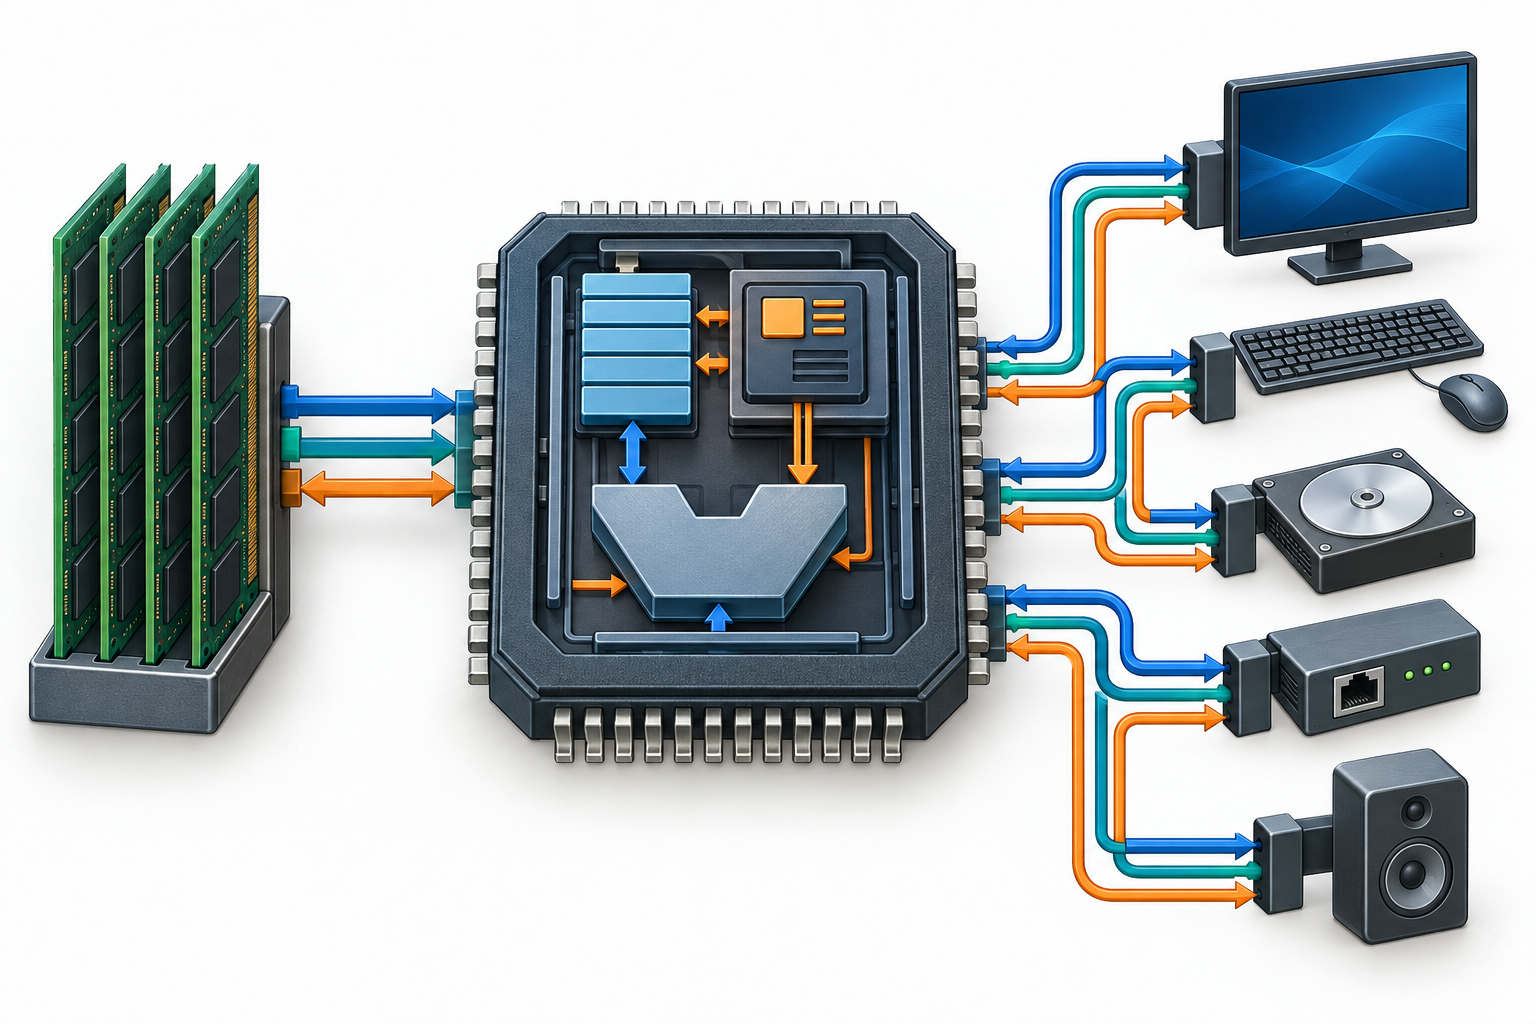
\includegraphics[width=\textwidth]{img/generated/cpu-architecture-generated.png}
\endobr{Zjednodušené propojení konfigurační vrstvy, simulačního jádra a periferií.}

\sekce{Procesor a~jeho vnitřní části}
Procesor lze z~hlediska mikroarchitektury rozdělit na datovou cestu a~řídicí jednotku. Datová cesta přenáší a~zpracovává hodnoty. Patří do ní především registrace, aritmeticko-logická jednotka, multiplexory, sběrnice a~rozhraní k~paměti. Řídicí jednotka určuje, která operace se v~daném okamžiku provede, které registry se čtou a~kam se zapíše výsledek.

Registry jsou velmi rychlé úložné prvky přímo uvnitř procesoru. Programový čítač uchovává adresu další instrukce. Instrukční registr může držet právě načtený bitový vzor. Ukazatel zásobníku ukazuje na vrchol zásobníku a~stavový registr uchovává informace o~předchozím výpočtu. Obecné registry slouží k~uchování operandů a~mezivýsledků.

ALU provádí aritmetické a~logické operace. Při sčítání může vzniknout přenos do vyššího bitu, při odčítání výpůjčka a~při práci se znaménkovými čísly přetečení rozsahu. Proto ALU kromě výsledku často vytváří stavové příznaky. Příznak Z označuje nulový výsledek, C přenos, O znaménkové přetečení a~N záporný výsledek. Procesor je může použít například při podmíněném skoku.

\obrazek
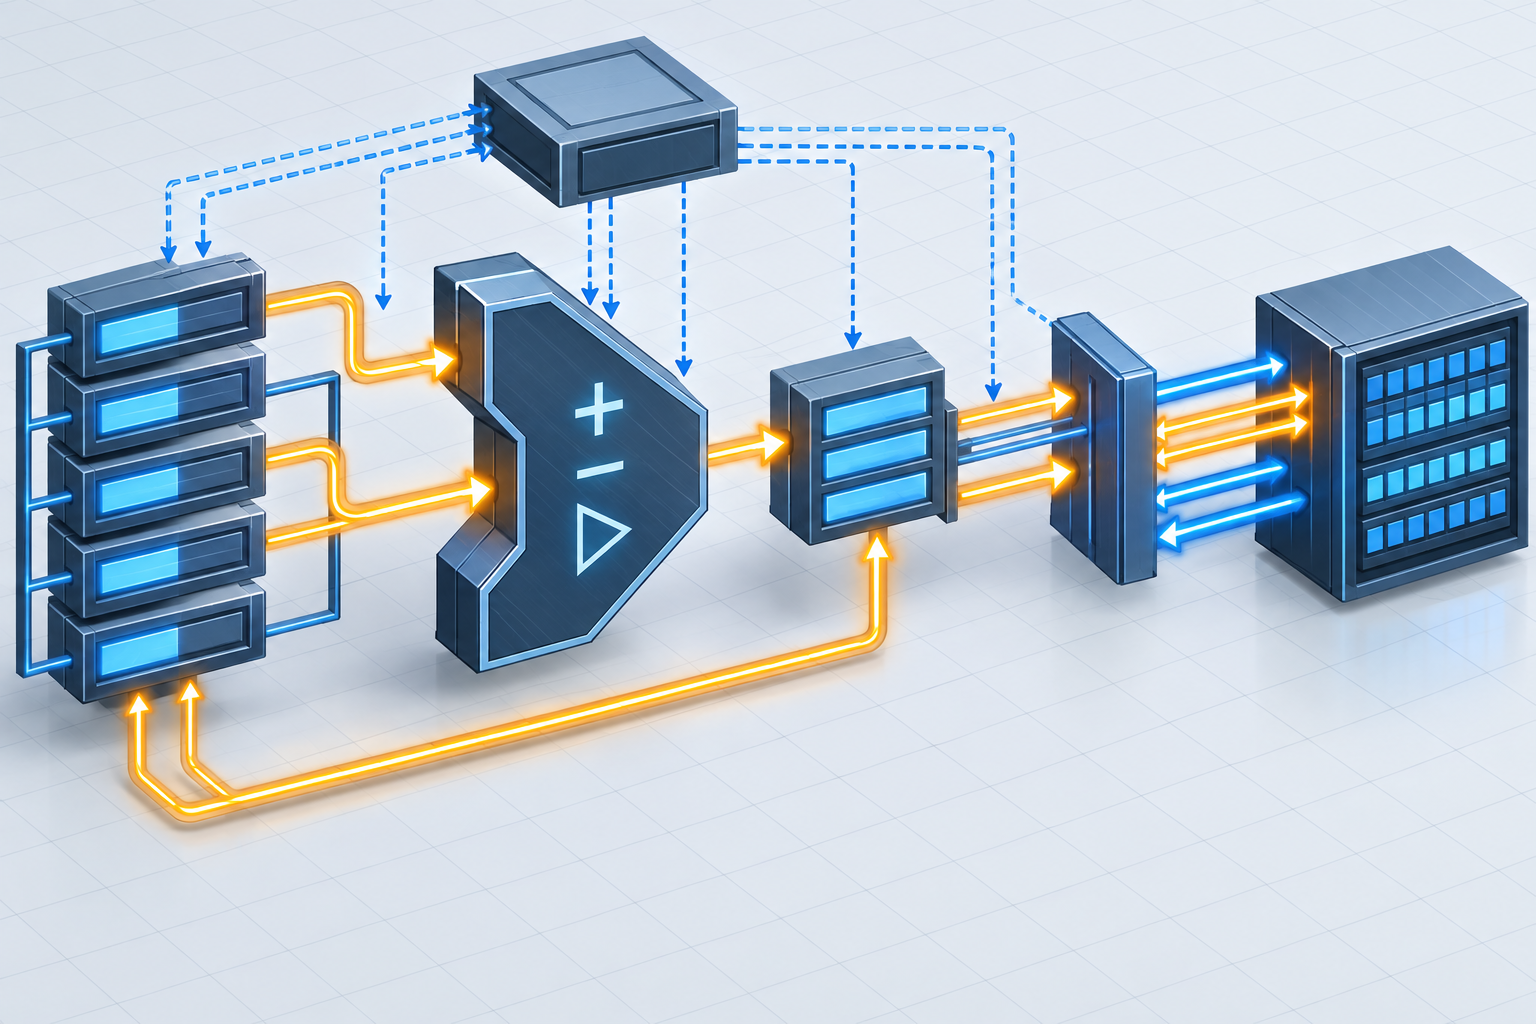
\includegraphics[width=\textwidth]{img/generated/cpu-datapath-generated.png}
\endobr{Datová cesta procesoru mezi čítačem instrukcí, registry, ALU, pamětí a periferiemi.}

\sekce{Instrukční sada a~mikroarchitektura}
Instrukční sada (ISA) je smlouva mezi programem a~procesorem. Určuje názvy nebo číselné kódy instrukcí, formát operandů, velikost dat a~viditelné registry. Mikroarchitektura popisuje, jak je ISA uvnitř procesoru realizována. Dvě zařízení mohou mít stejnou ISA, ale odlišnou datovou cestu, počet cyklů i~způsob řízení.

V~tomto projektu je hranice mezi ISA a~mikroarchitekturou záměrně viditelná v~konfiguračním souboru. Pole \texttt{encoding} popisuje vnější binární formát instrukce a~pole \texttt{microcode} popisuje její vnitřní provedení. Jedna instrukce tak může být složena z~několika jednoduchých kroků, například z~výpočtu nové hodnoty SP, zápisu na zásobník a~změny PC.

Mikrokód představuje posloupnost elementárních řídicích operací. Jeho výhodou je snadná popisnost složitějších instrukcí a~možnost sledovat jednotlivé kroky. Nevýhodou je režie spojená s~interpretací mikrooperací. V~tomto simulátoru je mikrokód zároveň součástí modelu: zpřístupňuje vnitřní přechody, ale jeho interpretovaná režie nepředstavuje časovou charakteristiku skutečného procesoru.

\sekce{Sběrnice a~přenos dat}
Sběrnice je sdílená komunikační cesta, po které se přenášejí hodnoty. Adresní sběrnice určuje místo, se kterým se pracuje, datová sběrnice přenáší samotná data a~instrukční cesta přenáší kód instrukce. Šířka sběrnice ovlivňuje množství bitů přenesených jedním krokem a~velikost hodnot, které lze přirozeně zpracovat.

Datový přenos lze z~modelového hlediska rozdělit do tří základních fází. Zdroj vloží hodnotu na datovou cestu, řídicí jednotka vybere cílový prvek a~cílový prvek hodnotu převezme. U~paměťové operace se nejprve nastaví adresa, následně se provede čtení nebo zápis a~nakonec se výsledek zapíše do registru. Skutečné procesory tyto činnosti realizují pomocí řídicích signálů; simulátor je vyjadřuje mikrooperacemi.

\sekce{Vykonávací cyklus instrukce}
Zpracování instrukce je v~simulátoru modelováno jako stavový přechod přes fáze načtení, dekódování a~provedení. Ve fázi načtení PC určí adresu instrukce a~instrukce se přenese z~paměti do interního stavu procesoru. PC se obvykle posune na další instrukci. Dekódování zjistí operační kód a~z~bitových polí vytvoří konkrétní hodnoty operandů.

Ve fázi provedení řídicí jednotka aktivuje datovou cestu podle mikroprogramu. Instrukce MOV například pouze přečte zdrojový registr a~zapíše jeho hodnotu do cílového registru. Instrukce ADD navíc aktivuje ALU a~může změnit FLAGS. Instrukce LOAD a~STORE používají adresní a~datovou sběrnici paměti. Po dokončení se stav procesoru ustálí a~cyklus začne znovu.

Počet hodinových cyklů nemusí odpovídat počtu instrukcí. Jedna instrukce může potřebovat více mikrooperací a~jedna mikrooperace může mít vlastní latenci. Simulátor proto rozlišuje dynamické časování a~režimy s~předepsaným časovým rozpočtem. Toto rozlišení umožňuje vysvětlit rozdíl mezi funkční správností instrukce a~její časovou náročností.

\obrazek
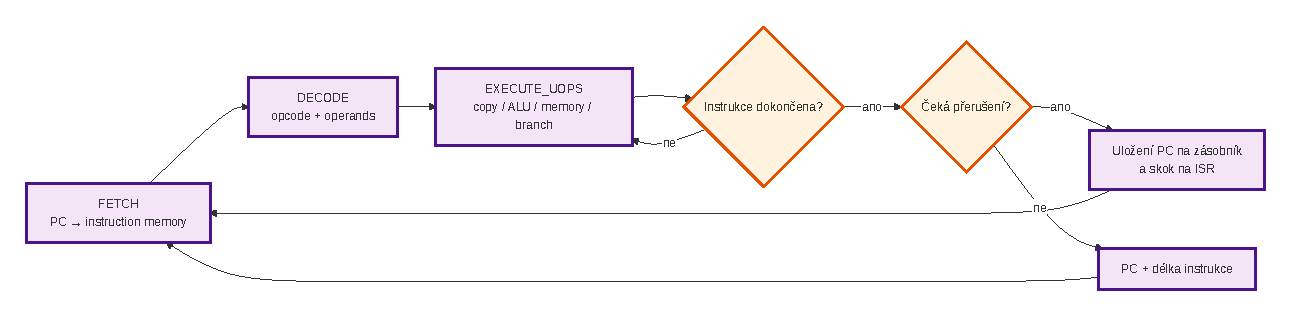
\includegraphics[width=\textwidth]{img/instruction-cycle.pdf}
\endobr{Stavy vykonávacího cyklu instrukce včetně zpracování přerušení.}

\sekce{Paměťová hierarchie a~ochrana}
Paměť procesoru je výrazně pomalejší než registry, ale nabízí mnohem větší kapacitu. V~reálných počítačích se proto používá hierarchie registrů, cache, operační paměti a~trvalého úložiště. Tento simulátor se soustředí na adresovatelnou paměť, instrukční prostor, datový prostor a~MMIO; neimplementuje fyzickou cache ani model elektrických zpoždění.

Oprávnění R, W a~X představují základní model ochrany. Čtení vyžaduje R, zápis W a~načtení instrukce X. Například ROM může mít povoleno čtení a~vykonávání, ale zakázaný zápis, zatímco RAM může být zapisovatelná a~nevykonatelná. Oddělení práv omezuje chyby programu a~zároveň názorně ukazuje rozdíl mezi daty a~kódem.

\obrazek
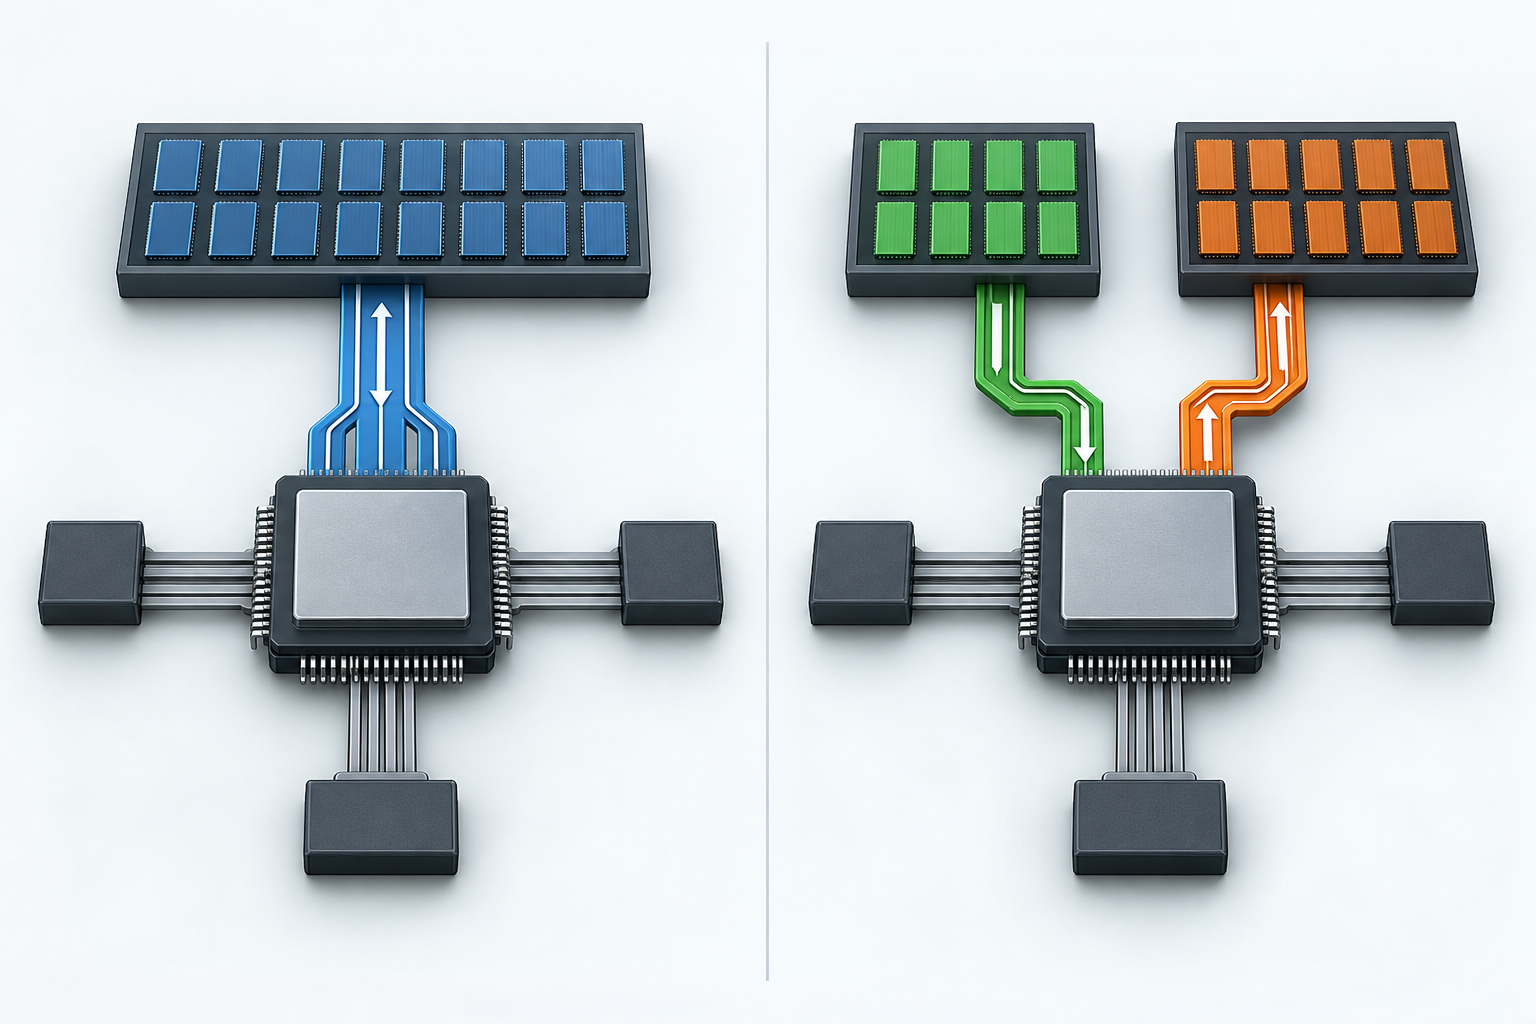
\includegraphics[width=\textwidth]{img/generated/memory-topology-generated.png}
\endobr{Porovnání sjednoceného a odděleného adresního prostoru paměti.}

\sekce{Periferie a~I/O}
Periferie jsou zařízení, která provádějí činnost mimo základní datovou cestu CPU. Patří sem klávesnice, displeje, časovače, sériová rozhraní, řadiče přímého přístupu do paměti a~koprocesory. Procesor s~nimi komunikuje pomocí definovaných registrů a~řídicích hodnot.

U~MMIO jsou řídicí registry periferie umístěny do části adresního prostoru. Instrukce STORE do této oblasti není obyčejný zápis do RAM, ale událost, která může například odeslat znak na terminál nebo spustit přenos DMA. Při čtení může zařízení vrátit aktuální stav, odebrat znak ze vstupního bufferu nebo vygenerovat novou náhodnou hodnotu.

Alternativou je port-mapped I/O, kde mají porty vlastní číselný prostor a~procesor používá speciální instrukce pro čtení a~zápis. Simulátor podporuje oba přístupy, což umožňuje porovnat jejich datový tok. Deklarativní model navíc ukazuje, že periferní zařízení lze popsat stavovým automatem tvořeným registry, podmínkami a~akcemi.

\obrazek
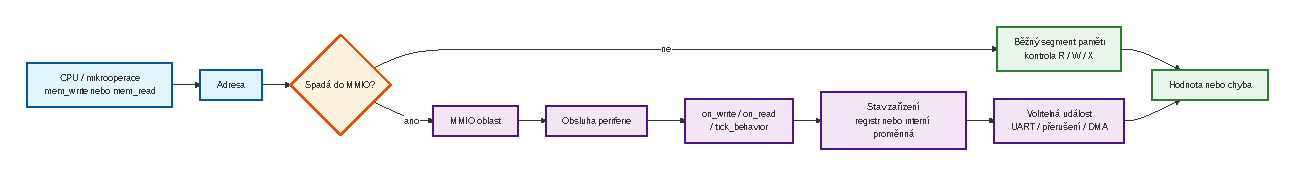
\includegraphics[width=\textwidth]{img/mmio-flow.pdf}
\endobr{Zpracování přístupu do paměťově mapované periferie.}

\sekce{Přerušení a~asynchronní události}
Přerušení představuje mechanismus asynchronní signalizace, kterým periferní zařízení mění řídicí tok procesoru bez periodického dotazování jeho stavu. Procesor uloží návratový kontext, načte adresu obslužné rutiny a~začne vykonávat její instrukce. Po dokončení obsluhy se návratová adresa obnoví ze zásobníku.

V~simulátoru je přerušení vektorizované a~executor při jeho zpracování automaticky uloží návratovou adresu na zásobník. Deklarativní periferie může přerušení vyvolat například po dokončení DMA přenosu. Tím lze zkoumat rozdíl mezi synchronní operací provedenou instrukcí a~asynchronní událostí vzniklou v~periferii.

\obrazek
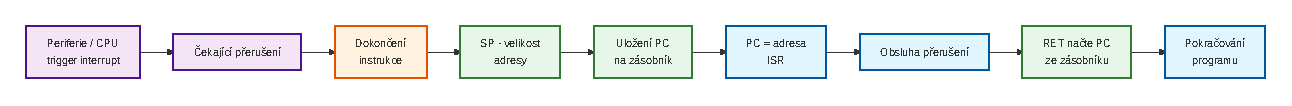
\includegraphics[width=\textwidth]{img/interrupt-lifecycle.pdf}
\endobr{Životní cyklus hardwarového přerušení od jeho vyvolání po návrat instrukcí RET.}
\kapitola{Návrh simulované architektury}
\sekce{Konfigurační princip}
Kořen konfiguračního souboru obsahuje název architektury, šířku datové a~adresové sběrnice, popis paměti, registry, ALU, instrukční sadu a~seznam periferií. Při spuštění aplikace metoda \texttt{Config::from\_file} JSON načte, převede jej na interní datové struktury a~zkontroluje jeho platnost. Simulátor proto nemusí znát konkrétní instrukční sadu předem \textsuperscript{[3]}.

Datová sběrnice určuje přirozenou šířku operací a~výchozí velikost slov. Adresová sběrnice určuje velikost adres a~šířku operandů typu \texttt{address}. Projekt podporuje šířky od 4 do 128 bitů v~násobcích čtyř. Aritmetika pracuje s~typem \texttt{word\_t}, jehož velikost umožňuje jednotné zacházení s~hodnotami v~celém jádře.
\obrazek
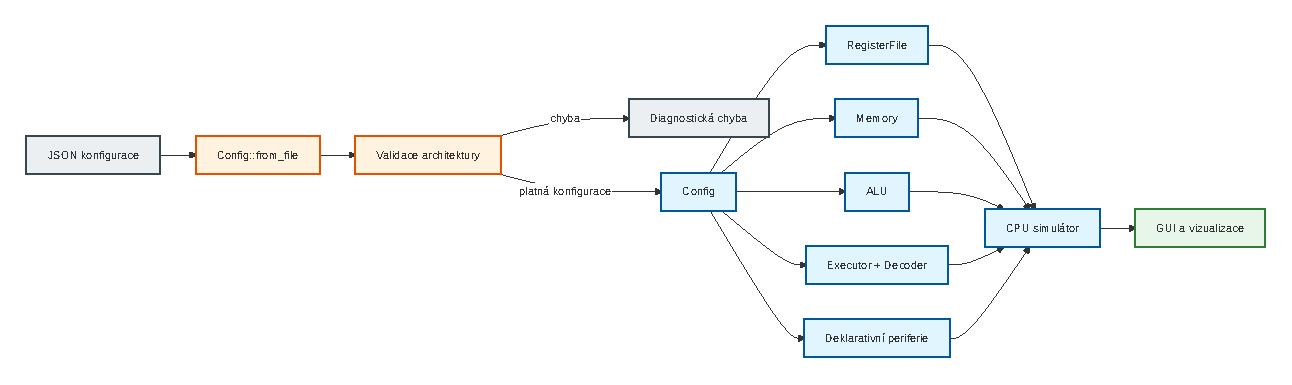
\includegraphics[width=\textwidth]{img/configuration-lifecycle.pdf}
\endobr{Životní cyklus konfigurace od JSON souboru po vytvoření CPU a vizualizaci.}
\sekce{Registry a~registr zásobníku}
Soubor registrů obsahuje fyzické registry a~speciální registry rozpoznávané podle role. Role programového čítače (PC) určuje adresu další instrukce, role ukazatele zásobníku (SP) řídí operace se zásobníkem a~role stavových příznaků (FLAGS) poskytuje podmínky pro větvení.

Registr může obsahovat podregistry. Kontinuální podregistr je určen šířkou a~bitovým posunem, zatímco maskovaný podregistr vybírá i~nesousedící bity. Čtení podregistru provede výřez z~fyzického registru; zápis použije operaci read-modify-write, takže neovlivní ostatní bity rodičovského registru. Stejný mechanismus lze použít i~hierarchicky.
\sekce{Aritmeticko-logická jednotka}
ALU nevykonává pouze pevně naprogramované operace. Každá operace je popsána jménem a~výrazem nad operandy \texttt{a}, \texttt{b} a~\texttt{c}. Výraz se při vytvoření ALU rozloží tokenizerem, převede Shuntingovým algoritmem do reverzní polské notace a~při vykonání se vyhodnotí. Lze tak definovat sčítání, odčítání, násobení, logické operace, posuny i~vlastní kombinace.

Po operaci může ALU upravit bity ve FLAGS. Vestavěná pravidla určují nulový výsledek, záporný výsledek, přenos, výpůjčku a~číselné přetečení. Konfigurace může místo vestavěného pravidla použít vlastní logický výraz s~výsledkem operace \texttt{res}. U~pomalejších operací lze nastavit počet cyklů, který se promítne do latence vykonávání.
\sekce{Paměť a~ochrana přístupu}
Paměť může používat sjednocený adresní prostor (Von Neumannova architektura), nebo oddělený prostor instrukcí a~dat (Harvardská architektura). Vícebajtové hodnoty se ukládají podle nastaveného pořadí bajtů, tedy little-endian nebo big-endian.

Adresní prostor je rozdělen na pojmenované segmenty. Každý segment má samostatná oprávnění ke čtení (R), zápisu (W) a~vykonávání (X). Kontrola probíhá při každém čtení, zápisu i~načtení instrukce. Pokus o~nepovolený přístup vyvolá diagnostickou chybu namísto tichého poškození stavu simulátoru. Vedle běžných paměťových oblastí může paměť obsahovat mapované I/O oblasti a~číslované porty.
\sekce{Instrukční sada a~kódování}
Instrukce je určena názvem, číselným operačním kódem, binárním kódováním a~seznamem mikrooperací. Kódování kombinuje pevná pole s~poli pro registry, okamžité hodnoty a~adresy. Dekodér z~bitového proudu nejprve podle operačního kódu vybere instrukci a~poté z~něj získá jednotlivé operandy.

Význam instrukce není pevně zakódován v~programu. Její chování popisuje mikrokód, jehož mikrooperace mohou kopírovat hodnoty, spouštět ALU, číst a~zapisovat paměť, pracovat s~porty nebo koprocesorem, větvit tok programu a~zastavit procesor. Operandové značky mají jednoznačný význam: \texttt{@} odkazuje na operand aktuální instrukce, \texttt{\$} na speciální registr a~\texttt{\#} na konstantu.

\obrazek
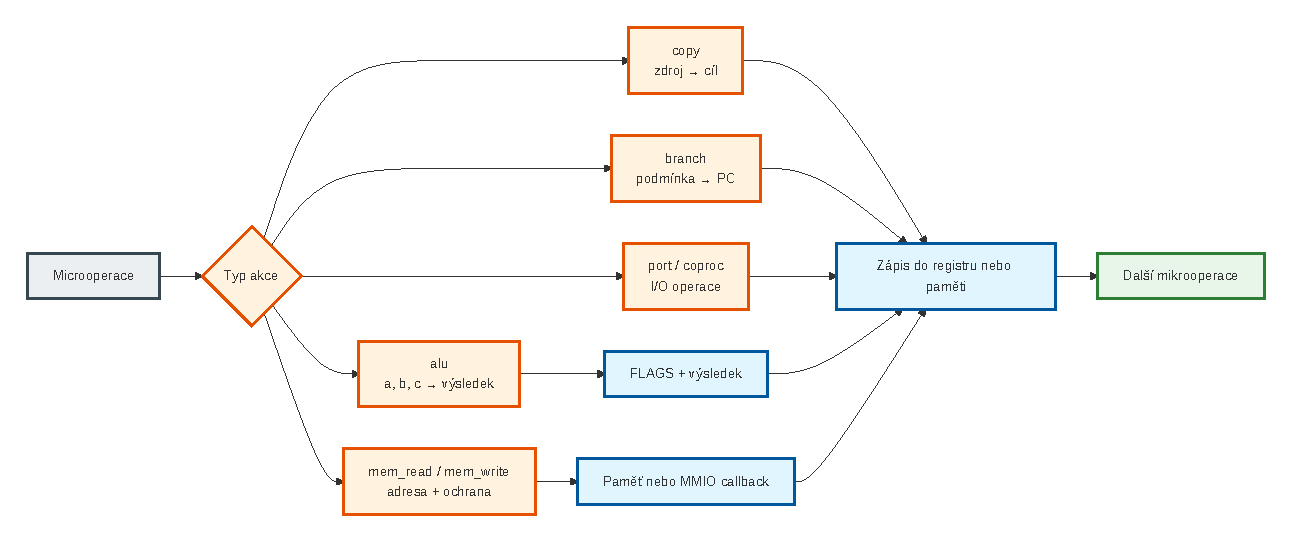
\includegraphics[width=\textwidth]{img/microoperation-path.pdf}
\endobr{Typy mikrooperací a jejich cesta k zápisu výsledku do stavu procesoru.}
\sekce{Řídicí jednotka a~časování}
Executor je stavový automat se stavy \texttt{FETCH}, \texttt{DECODE}, \texttt{EXECUTE\_UOPS} a~\texttt{DONE}. Ve fázi FETCH načte instrukci z~adresy PC, ve fázi DECODE ji dekodér rozloží a~ve fázi EXECUTE\_UOPS executor postupně provede její mikrooperace. Po dokončení se řízení vrátí do FETCH.

Metoda \texttt{CPU::step} provede jednu celou instrukci. Jemnější metoda \texttt{CPU::step\_uop} provede právě jednu mikrooperaci a~umožňuje zkoumat jednotlivé přechody stavu. Po každé mikrooperaci se aktualizuje stav periferií. Časování může být dynamické, pevné (strict), určené úzkým hrdlem (bottleneck) nebo aditivní. Tyto režimy porovnávají varianty abstraktního modelu; nejde o~měření ani predikci fyzického hardwaru.

Procesor podporuje také vektorizovaná přerušení. Při přijetí přerušení executor uloží návratovou adresu na zásobník a~nastaví PC na adresu obslužné rutiny. Návrat se provede instrukcí \texttt{RET}, stejně jako u~běžného volání podprogramu.

\kapitola{Periferní zařízení}
\sekce{Princip komunikace s~periferiemi}
Periferie rozšiřují počítač o~zařízení, která nejsou součástí registrů ani hlavní paměti. Procesor s~nimi komunikuje stejně jako s~adresovým prostorem: speciální oblast adresy je přesměrována na čtení nebo zápis zařízení. Tento princip se nazývá memory-mapped I/O (MMIO). Simulátor podporuje také samostatné číslované porty a~přístup ke koprocesorovým registrům.

Každá periferie má jméno, typ a~rozsah adres. Deklarativní periferie navíc obsahuje interní stav, registry a~seznam akcí spouštěných při čtení, zápisu nebo taktu. Akce tvoří jednoduchý abstraktní syntaktický strom: mohou přiřazovat hodnoty, vyhodnocovat podmínky, volat hostitelské funkce a~číst nebo zapisovat systémovou paměť.
\sekce{Dostupné typy periferií}
Projekt rozlišuje několik typů zařízení:
\begin{itemize}
\item \textbf{textový displej nebo UART} přijímá bajty zapsané do MMIO registru a~předává je terminálu aplikace;
\item \textbf{deklarativní zařízení} umožňuje vytvořit vlastní registry a~logiku bez úprav C++ kódu;
\item \textbf{časovač} zvyšuje registr při každém taktu procesoru;
\item \textbf{vstupní zařízení} poskytuje hostitelský vstup podle konkrétní konfigurace;
\item \textbf{mřížkový displej} slouží k~zobrazení stavů LED nebo jiné jednoduché matice;
\item \textbf{koprocesor} může být ovládán vlastními registry přes mikrooperace \texttt{coproc\_read} a~\texttt{coproc\_write}.
\end{itemize}

V~aktuální implementaci jsou textové a~deklarativní periferie připojeny přímo na paměťově mapovanou I/O sběrnici. Mřížkový displej a~některé vstupní prvky jsou zatím vizualizovány jako widgety v~panelu periferií a~nepředstírají přímé čtení z~procesorové paměti. Toto rozlišení je důležité při interpretaci validačních výsledků.
\sekce{Příklad deklarativního zařízení}
Konfigurace může definovat matematický koprocesor se vstupními registry \texttt{OP\_A} a~\texttt{OP\_B}, výstupním registrem \texttt{RESULT} a~řídicím registrem \texttt{CMD}. Zápis hodnoty 1 do CMD může vyvolat násobení a~zápis hodnoty 2 dělení. Procesor tedy zařízení nevolá pomocí pevné implementace, ale běžným zápisem do adresního prostoru.

Jiný příklad představuje DMA řadič s~registry zdrojové adresy, cílové adresy, velikosti přenosu, řídicího slova a~stavu. Při každém taktu může přečíst slovo ze zdroje, případně je upravit pomocí XOR klíče, zapsat je do cíle a~posunout adresy. Po dokončení může vyvolat přerušení. Deklarativní model tak umožňuje popsat i~stavové zařízení, aniž by bylo nutné vytvářet novou třídu.

\kapitola{Assembler a~průběh vykonání programu}
\sekce{Assembler}
Assembler zpracovává zdrojový text ve více průchodech. V~prvním průchodu rozdělí řádky na tokeny a~zachytí návěští. V~dalším průchodu podle definice instrukce zkontroluje typy operandů, dosadí adresy návěští a~vytvoří strojový kód. Očekávané formáty operandů odvozuje ze stejného pole \texttt{encoding}, které používá dekodér, takže assembler a~vykonávací část sdílejí popis instrukcí.
\obrazek
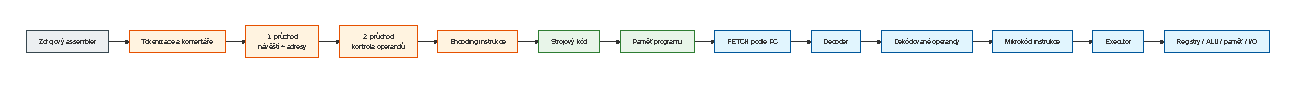
\includegraphics[width=\textwidth]{img/assembler-decoder.pdf}
\endobr{Společná cesta od zdrojového assembleru přes kódování a dekódování až k vykonání mikrooperací.}
\sekce{Modelový průchod instrukce}
Při instrukci typu \texttt{LOAD} se nejprve načte operační kód a~zvýší se PC. Dekodér z~dalších bitů získá cílový registr a~zdroj adresy. Mikrokód následně provede mikrooperaci \texttt{mem\_read}, paměť zkontroluje oprávnění a~vrácenou hodnotu zapíše do cílového registru. Při čtení MMIO adresy se místo běžné paměti zavolá obsluha příslušné periferie.

U~aritmetických instrukcí se operandy předají ALU. Ta vyhodnotí nakonfigurovaný výraz, výsledek ořízne na šířku operandu a~podle pravidel aktualizuje FLAGS. Podmíněné větvení pak příznak přečte a~buď nastaví PC na cílovou adresu, nebo pokračuje další instrukcí. U~instrukcí \texttt{CALL}, \texttt{RET}, \texttt{PUSH} a~\texttt{POP} se navíc pracuje se SP a~paměťovou oblastí zásobníku.

\kapitola{Implementace desktopové aplikace}
\sekce{Struktura programu}
Simulační jádro je odděleno od uživatelského rozhraní. Adresář \texttt{src/core} obsahuje konfiguraci, CPU, ALU, assembler, dekodér, executor, paměť, registry a~periferie. Adresář \texttt{src/ui} obsahuje jednotlivé panely grafického rozhraní. Funkce \texttt{main} připraví konfiguraci, vytvoří CPU, inicializuje periferie a~spustí hlavní smyčku.

Grafické rozhraní používá SDL2 pro okno a~zpracování událostí, OpenGL pro vykreslování a~Dear ImGui pro tvorbu panelů. Rozhraní obsahuje řídicí panel, zobrazení registrů, monitor ALU, prohlížeč paměti a~Flash ROM, průzkumník zásobníku, pipeline mikrooperací, assembler, programový pohled, panel periferií a~systémové schéma \textsuperscript{[4--6]}.

\obrazek
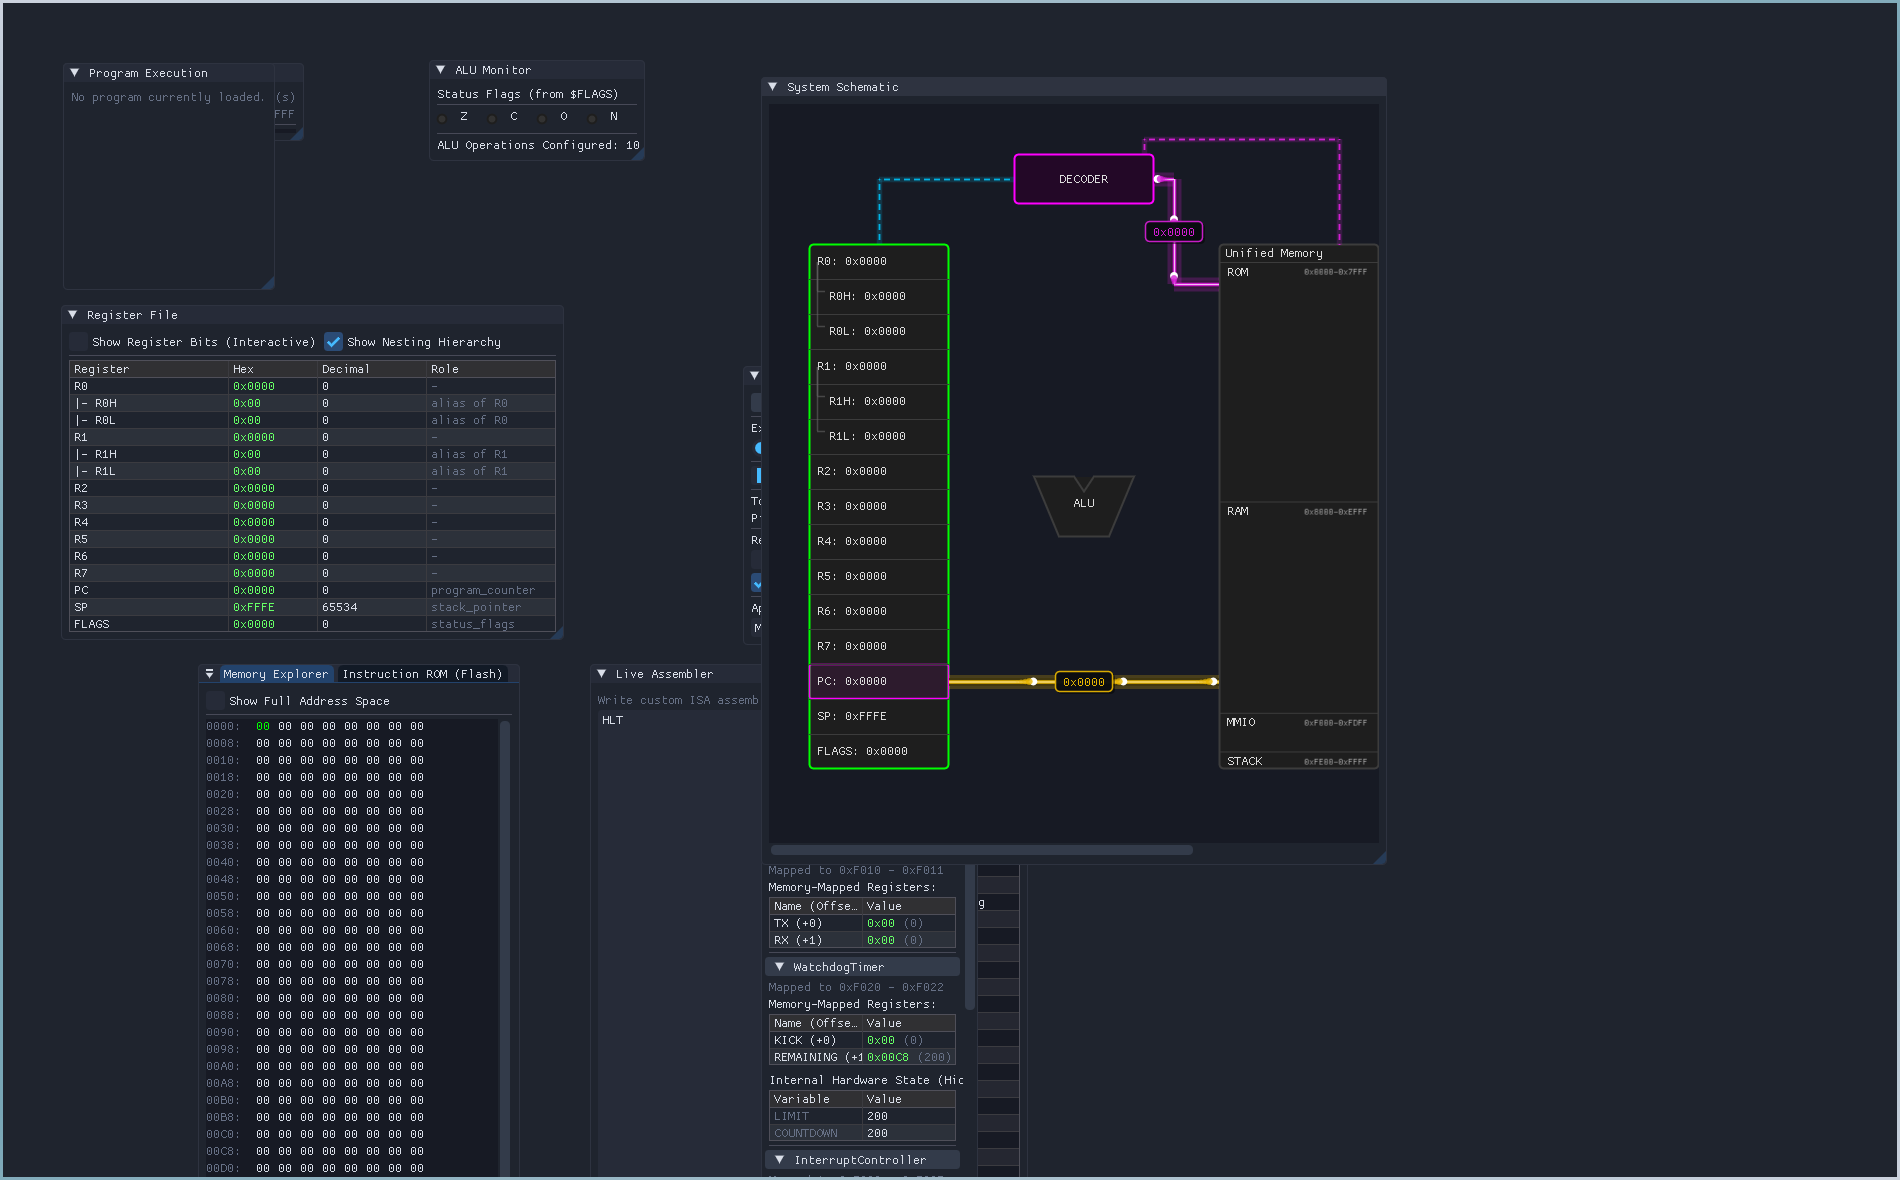
\includegraphics[width=\textwidth]{img/screenshots/simulator-16bit-overview.png}
\endobr{Běh hotového simulátoru s 16bitovou konfigurací RISC Lab.}

\obrazek
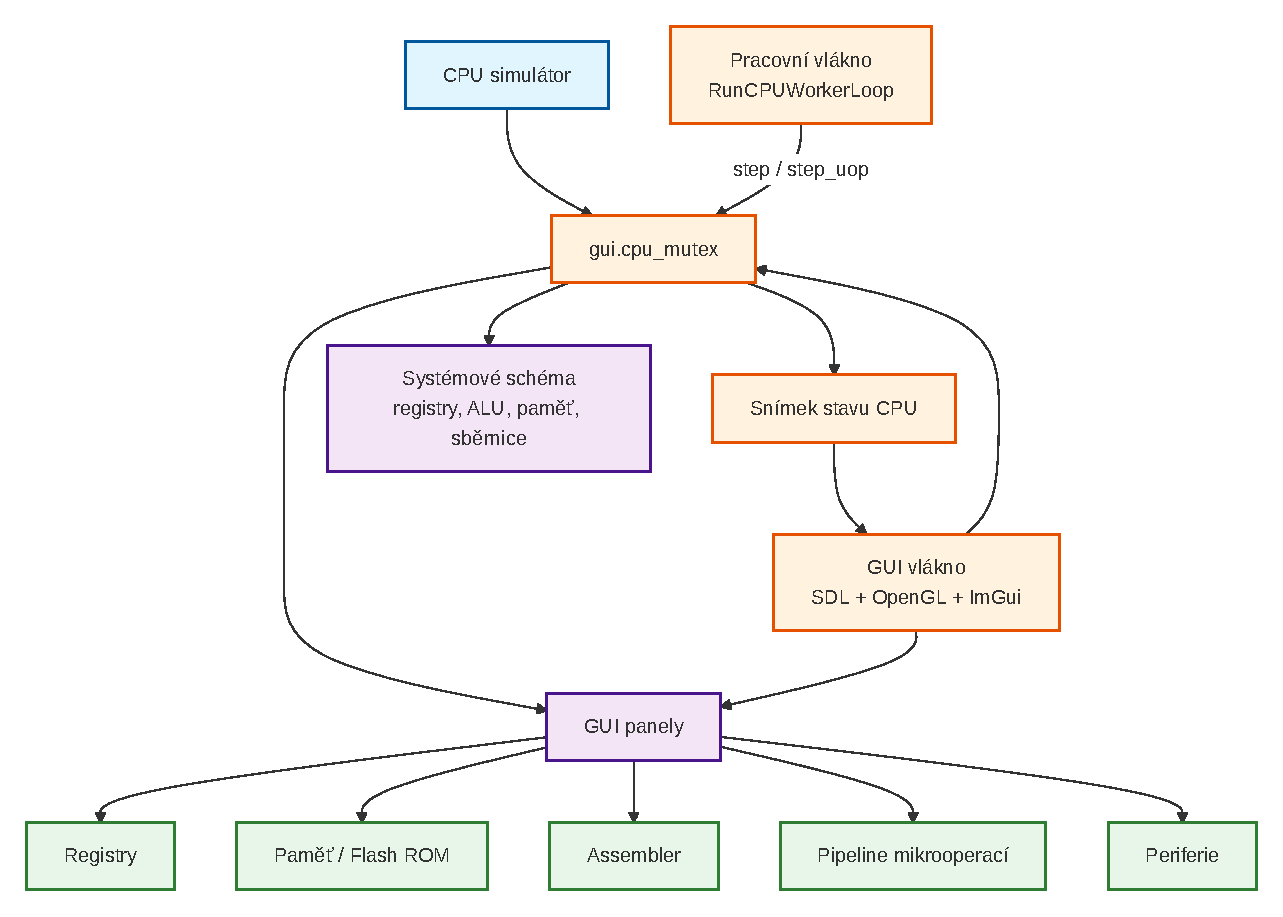
\includegraphics[width=\textwidth]{img/gui-system.pdf}
\endobr{Rozdělení aplikace na simulační vlákno, GUI vlákno, synchronizaci a zobrazovací panely.}
\sekce{Hlavní smyčka a~souběžné vykonávání}
Vykonávání CPU běží ve vlákně odděleném od vlákna grafického rozhraní. Sdílený stav je chráněn mutexem, aby se nemohlo současně zapisovat do CPU z~vykonávacího vlákna a~číst z~něj při vykreslování. Rychlost hodin lze řídit z~řídicího panelu; uživatel může spustit program, pozastavit jej, provést instrukci nebo provést jednu mikrooperaci.
\sekce{Vizualizace datové cesty}
Struktura systému zobrazuje registry, dekodér, ALU, paměť a~periferie jako bloky propojené adresní, datovou a~instrukční sběrnicí. Pomocný objekt \texttt{BusHighlighter} podle aktuální mikrooperace určí aktivní trasu a~její intenzitu. Aktivní spojení se animuje, takže uživatel vidí nejen výsledný stav registrů, ale i~cestu právě přenášené hodnoty.

Aplikace udržuje snímky stavu CPU. Díky nim lze procházet historii běhu, sledovat změny registrů a~vracet se k~dřívějšímu okamžiku simulace. Samostatné panely zobrazují čísla v~hexadecimální, desítkové i~bitové podobě a~zvýrazňují PC, SP, aktivní mikrooperaci a~body zastavení.
\sekce{Konfigurace a~spuštění}
Po překladu se simulátor spouští s~cestou ke konfiguračnímu souboru, například:
\begin{verbatim}
./cpu_sim ../configs/8bit.json
\end{verbatim}
Při načtení se konfigurace nejprve syntakticky zpracuje a~poté ověří. Pokud je architektura neplatná, aplikace vypíše diagnostickou chybu a~CPU nevytvoří. Konfigurační soubory v~projektu představují například 4bitový, 8bitový a~16bitový procesor; jeden z~8bitových návrhů používá oddělenou instrukční a~datovou paměť.

\obrazek
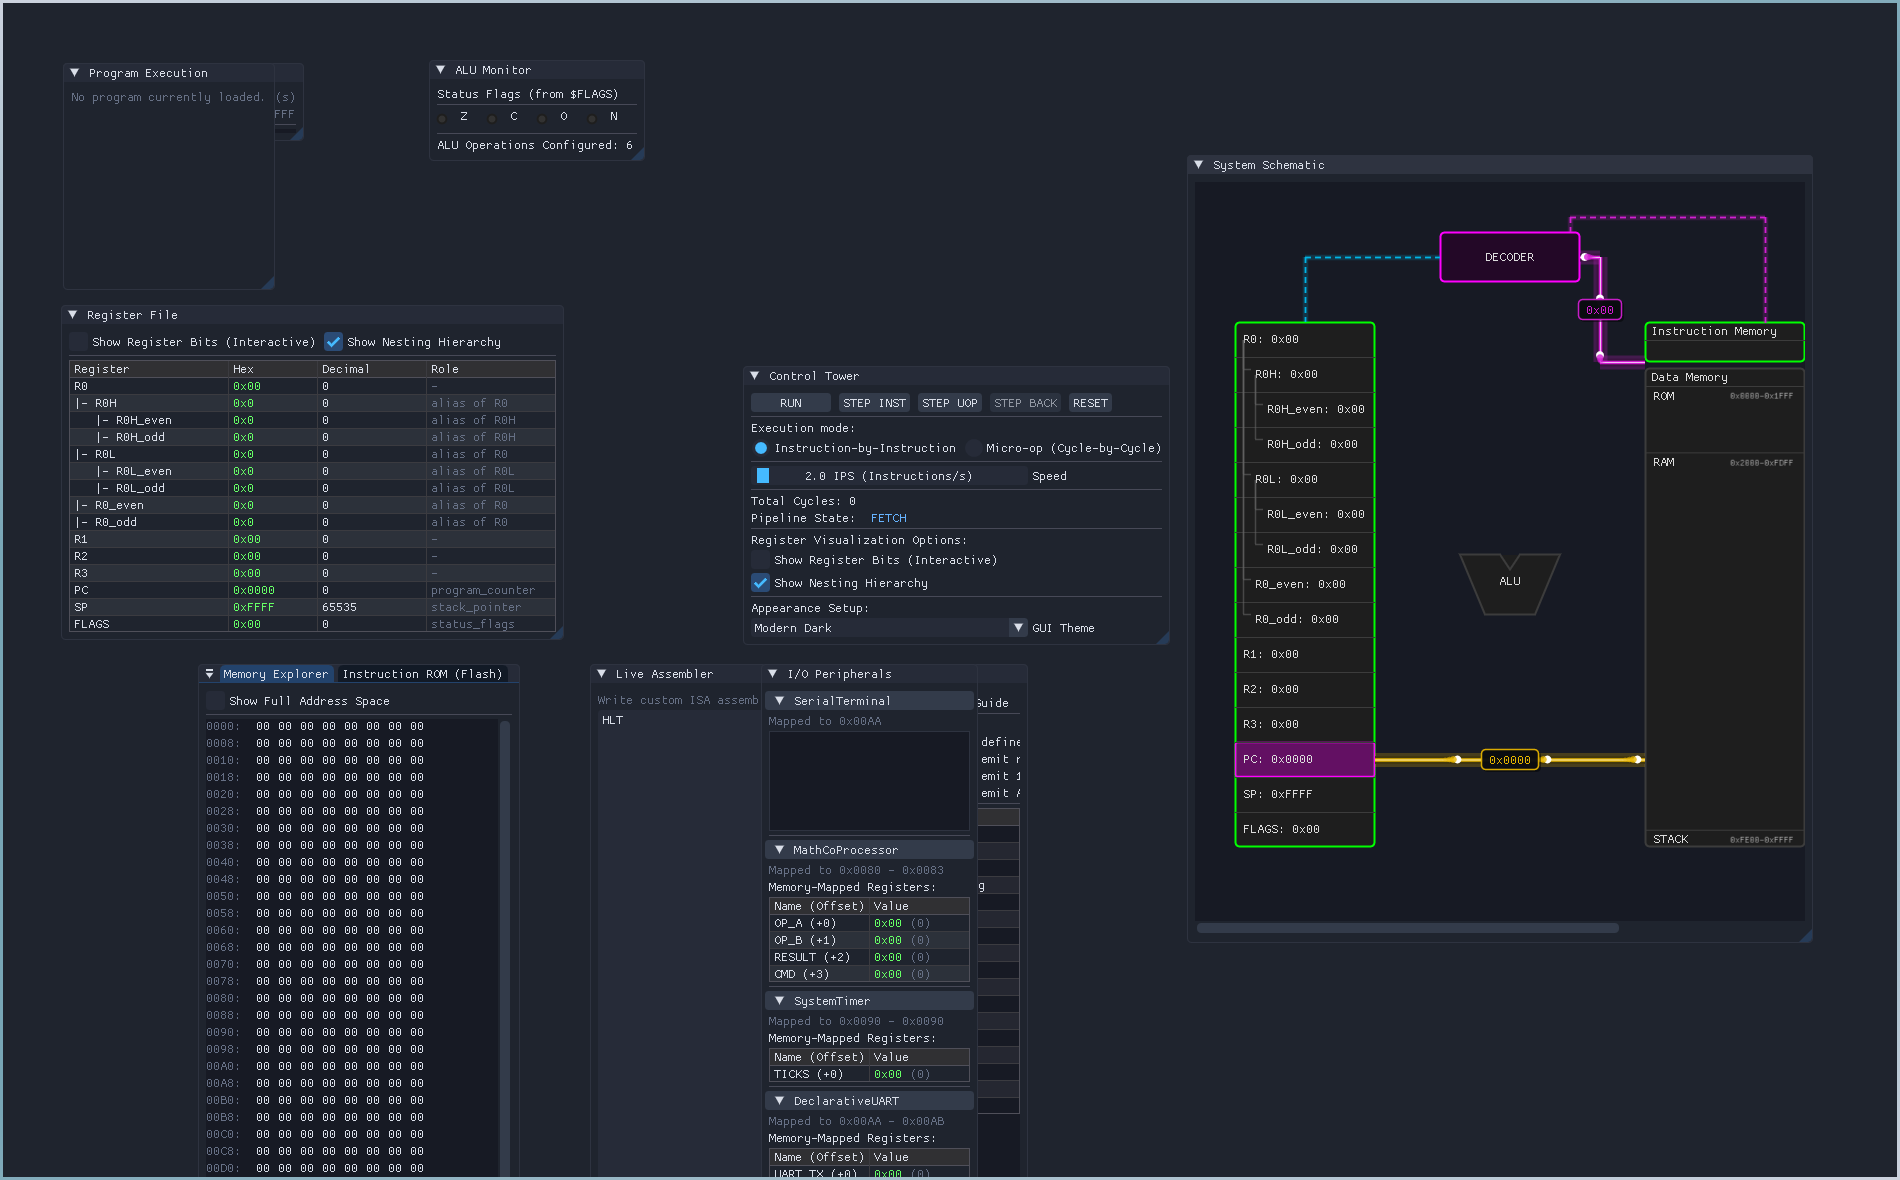
\includegraphics[width=\textwidth]{img/screenshots/simulator-8bit-harvard.png}
\endobr{Experimentální konfigurace simulátoru s 8bitovou Harvardskou architekturou a oddělenými prostory instrukcí a dat.}

\sekce{Praktická realizace simulačního jádra}
Simulační jádro je implementováno v~jazyce C++ a~je navrženo tak, aby jeho části měly jednoznačné odpovědnosti. Třída \texttt{Config} představuje načtený návrh hardwaru. Třída \texttt{CPU} propojuje registraci, paměť, ALU a~executor. Executor řídí pořadí operací, ale neobsahuje konkrétní instrukce; ty získává z~konfigurace.

Při konstrukci CPU se nejprve vytvoří soubor registrů, paměť, ALU a~vykonávací jednotka. Poté se pro každou deklarativní periferii zaregistrují obsluhy jejího adresního rozsahu do paměti. Díky tomu nemusí paměť znát konkrétní typ zařízení. Při přístupu pouze vyhledá oblast a~předá operaci odpovídající callback funkci.

\sekce{Parser a~validace konfigurace}
Načtení konfigurace se skládá ze dvou odlišných kroků. Parser převádí JSON hodnoty do struktur, zatímco validační část kontroluje, zda jejich kombinace dává smysl. Samostatná validace je důležitá například proto, že syntakticky správný JSON může obsahovat překrývající se segmenty, neplatnou šířku registru nebo instrukci s~nedosažitelným operačním kódem.

Kontrolují se šířky sběrnic, rozsahy adres, názvy a~role registrů, bitové posuny podregistrů, oprávnění segmentů, formáty instrukcí a~odkazy na existující ALU operace. U~periferií se ověřuje rozsah adres, velikost registrů a~platnost deklarovaných akcí. Při chybě program vypíše popis problému a~ukončí se před vytvořením grafického okna.

\sekce{Implementace souboru registrů}
Soubor registrů uchovává hodnoty fyzických registrů a~mapu jejich jmen. Při čtení je nejprve nalezen odpovídající fyzický registr. Pokud požadované jméno označuje alias, hodnota se posune a~zamaskuje podle definice podregistru. Zápis probíhá opačně: nová hodnota se ořízne na šířku aliasu, posune se na správné místo a~sloučí se s~hodnotou rodiče.

Vyhledávání podle role je důležitější než pevné indexy. Executor proto nepočítá s~tím, že PC bude vždy například prvním registrem. Konfigurace může pořadí registrů změnit a~role přesto zachová význam programového čítače, zásobníku a~příznaků. Tento návrh zvyšuje přenositelnost konfigurací.

\sekce{Implementace paměti a~MMIO}
Paměť ukládá hodnoty po bajtech a~při čtení nebo zápisu skládá vícebajtová slova podle nastaveného endianity. Před každou operací určí segment, zkontroluje typ přístupu a~teprve potom pracuje s~datovým úložištěm. Instrukční čtení používá příznak vykonávání, zatímco běžné datové čtení používá příznak čtení.

MMIO oblasti jsou uloženy v~samostatné mapě callbacků. Čtení nebo zápis v~jejich rozsahu se tedy neprovede v~běžném poli paměti. Periferie může přístup zpracovat okamžitě, změnit vlastní stav, vyvolat hostitelskou akci nebo vrátit aktuální hodnotu registru. Porty mají samostatnou tabulku, takže nekolidují s~adresami MMIO.

\sekce{Dekodér a~resolver operandů}
Dekodér si při vytvoření sestaví mapu bitového rozložení pro každý operační kód. Literálová pole porovnává s~načteným bitovým vzorem, zatímco pojmenovaná pole uloží do struktury dekódované instrukce. Registry se převádějí na jejich indexy a~okamžité hodnoty na číselné operandy.

Executor následně řeší operandové značky. Značka \texttt{@dest} odkazuje na operand získaný dekodérem, \texttt{\$PC} na registr s~rolí programového čítače a~\texttt{\#WORD\_SIZE} na konstantu odvozenou z~konfigurace. Stejný resolver se používá při čtení i~zápisu, čímž se omezuje počet míst, kde může vzniknout chyba v~interpretaci mikrokódu.

\sekce{Executor jako stavový automat}
Executor uchovává aktuální stav, načtený bitový vzor, dekódovanou instrukci, index mikrooperace, počitadla cyklů a~informaci o~zastavení. Metoda \texttt{step\_uop} posune automat právě o~jeden simulační krok. Metoda \texttt{CPU::step} ji volá opakovaně, dokud se nedokončí celá instrukce.

Akce \texttt{copy} přesouvá hodnotu mezi operandy. Akce \texttt{alu} načte operandy, zavolá ALU a~zapíše výsledek. Akce \texttt{mem\_read} a~\texttt{mem\_write} pracují s~pamětí, zatímco \texttt{port\_read} a~\texttt{port\_write} používají portové rozhraní. Větvení kontroluje příznak podle jeho jména nebo typu. Akce \texttt{halt} nastaví stav zastavení.

Před vlastním provedením se pro uživatelské rozhraní připravují diagnostické hodnoty. Ty umožní zobrazit předpokládanou adresu, vstup ALU nebo přenášená data, aniž by diagnostický náhled předčasně spustil vedlejší účinek MMIO čtení. Skutečný přístup k~periferii nastane až při provedení mikrooperace.

\sekce{Časování mikrooperací}
Každá ALU operace může mít vlastní latenci. Executor podle ní vytváří prodlevu, během které se mění počítadlo cyklů, ale neprovádí se opakovaně stejný vedlejší účinek. U~instrukce s~režimem dynamic odpovídá délka provedení přirozenému počtu mikrooperací a~latenci jejich funkčních jednotek.

Režim strict vynutí přesně nastavený počet cyklů. Pokud je mikrooperací málo, přidá prázdné cykly; pokud je jich mnoho, rozdělí nebo sloučí jejich vykonání podle dostupného časového rozpočtu. Bottleneck použije delší z~instrukčního rozpočtu a~reálné délky mikrooperací. Additive připojí pevnou režii až za dynamickou posloupnost. Tyto režimy jsou užitečné při porovnání různých návrhů stejné instrukční sady.

\sekce{Implementace deklarativních periferií}
Deklarativní periferie při vytvoření načte definice interních registrů a~stavových proměnných. Pro události \texttt{on\_read}, \texttt{on\_write} a~\texttt{tick\_behavior} vytvoří interpretovatelné uzly. Při události se uzly vyhodnocují v~pořadí daném konfigurací.

Výrazový parser podporuje literály, názvy registrů, aritmetické a~bitové operátory, porovnání a~logické podmínky. Akce přiřazení mění lokální stav periferie, podmíněná akce vybírá větev a~hostitelské volání propojuje simulované zařízení s~aplikací. Callback \texttt{host\_print} může například odeslat bajt do virtuálního terminálu, zatímco \texttt{sys\_read} a~\texttt{sys\_write} umožňují modelovat DMA.

\sekce{Implementace assembleru}
Assembler nejprve odstraní komentáře a~rozpozná návěští. V~prvním průchodu zjistí délku každého řádku podle encodingu instrukce a~získá adresy návěští. Ve druhém průchodu zkontroluje počet a~typ operandů, vyřeší symbolické adresy a~zapíše výsledná pole do strojového slova.

Assembler používá šířku datové a~adresové sběrnice z~konfigurace. Díky tomu se stejný zdrojový program může lišit délkou okamžitých hodnot nebo adres podle cílové architektury. Chybové stavy, například neznámá instrukce, chybějící návěští, hodnota mimo rozsah nebo neplatný registr, jsou vráceny grafickému panelu a~nevedou k~nahrání neúplného programu.

\sekce{Praktická práce s~aplikací}
Experimentální scénář začíná volbou konfiguračního souboru. Po jeho načtení může v~assembleru napsat krátký program a~nechat jej přeložit. Přeložená data se zobrazí v~programovém pohledu a~paměťovém panelu. Řídicí panel umožňuje procesor spustit, pozastavit nebo krokovat.

\obrazek
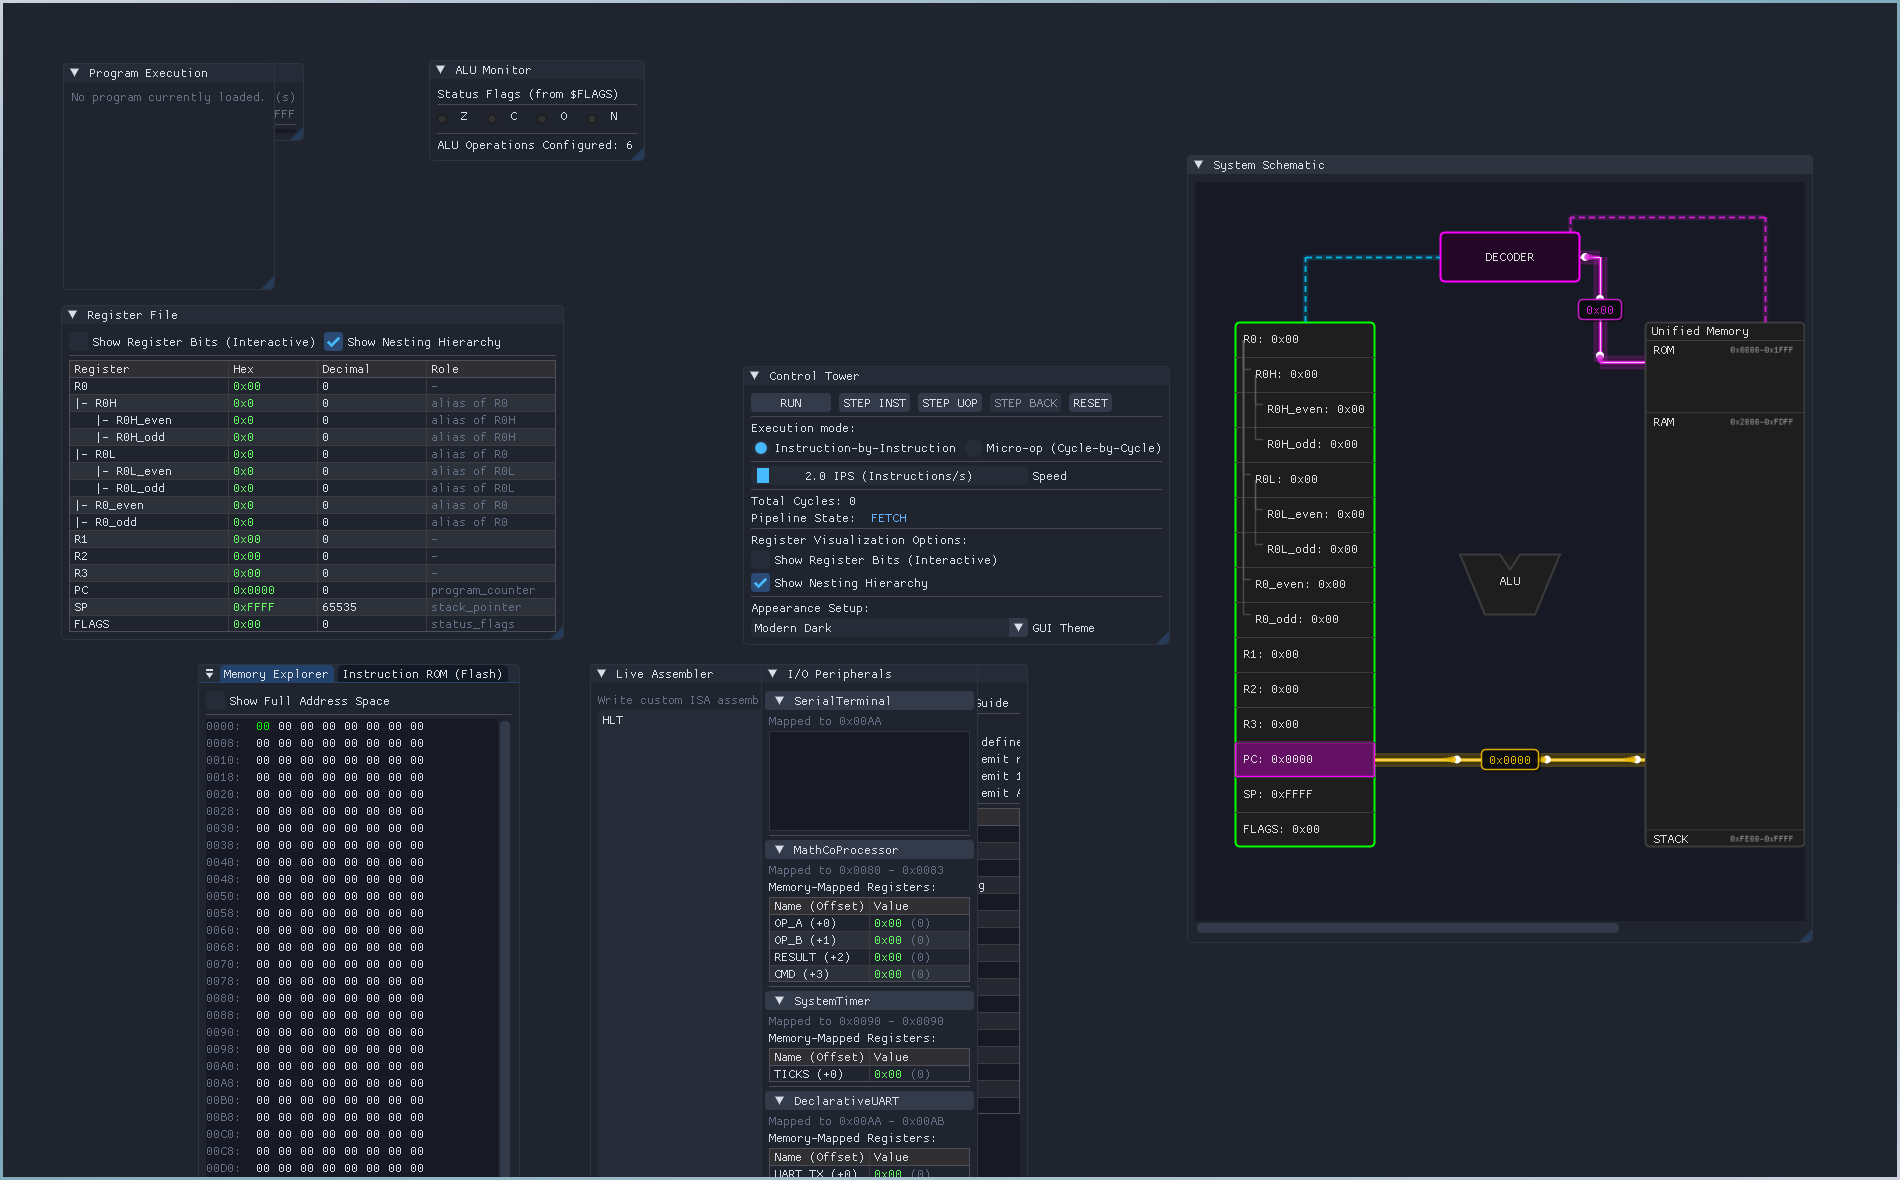
\includegraphics[width=\textwidth]{img/screenshots/simulator-8bit-vonneumann.png}
\endobr{Experimentální konfigurace simulátoru s 8bitovou Von Neumannovou architekturou, registry, prohlížečem paměti a panelem periferií.}

Krokování po instrukcích je vhodné pro sledování algoritmu. Krokování po mikrooperacích je vhodné pro sledování hardwarového průběhu. Při každém kroku lze porovnat hodnotu registrů, FLAGS, PC, SP, aktivní adresu, data na sběrnici a~stav periferií. Uživatel tak může například přesně určit okamžik, kdy instrukce STORE vyvolá změnu v~UART.

\sekce{Souběžnost a~správa stavu GUI}
Grafické vlákno zpracovává události SDL a~vykresluje ImGui. Samostatné pracovní vlákno posouvá CPU podle nastavené rychlosti. Přístup k~CPU chrání mutex, který zabraňuje současnému čtení a~zápisu z~obou vláken. Při ukončení aplikace GUI nastaví příznak zastavení a~počká na dokončení pracovního vlákna.

Sdílená struktura \texttt{GUIState} uchovává rychlost hodin, režim běhu, body zastavení, aktivní motiv, stav zvýraznění sběrnic a~historii snímků. Snímek obsahuje potřebné hodnoty CPU a~stav periferií. Historie umožňuje procházet předchozí stav a~vrátit se k~němu bez opětovného spuštění celého programu.

\kapitola{Ověření funkčnosti}
\sekce{Testovací strategie}
Každá důležitá část jádra má vlastní testovací program. Parser konfigurace ověřuje načítání registrů, ALU a~instrukcí. Test registrů kontroluje aliasy, bitové posuny a~masky. Test paměti ověřuje endianness, hranice segmentů a~chyby při porušení oprávnění. Další testy pokrývají dekodér, assembler a~integrační průchod procesoru.

Testy se sestavují pomocí CMake a~spouštějí přes CTest. Integrační testy kombinují konfiguraci, registry, paměť, dekodér a~executor, takže mohou odhalit chybu vzniklou až při spolupráci několika modulů. Kromě automatických testů je vhodné ověřit také interaktivní aplikaci: načíst konfiguraci, sestavit krátký program, provést jej po mikrooperacích a~zkontrolovat registry, paměť, příznaky i~výstup periferií.
\sekce{Validační metodika a reprodukovatelnost}
Pro ověření hlavního tvrzení práce byl doplněn samostatný nástroj \texttt{cpu\_validate}. Ten načte stejnou JSON konfiguraci a~zdrojový program v~assembleru jako grafická aplikace, vykonává CPU po jednotlivých simulačních krocích a~zapíše strojově čitelný JSON výsledek. Výsledek obsahuje konfiguraci, počet kroků a~cyklů, konečný stav registrů a~volitelný sled stavů. Každý scénář má předem určené hodnoty registrů; nesoulad ukončí běh chybou.

Validační matice obsahuje šest krátkých scénářů. Čtyřbitová konfigurace ověřuje aritmetiku registrů s~výsledkem \texttt{A=4} za sedm kroků. Osmibitový program vyvolá přetečení \texttt{250+10}, takže ověřuje \texttt{R0=4} a~příznak přenosu \texttt{FLAGS=2}; stejný program je spuštěn pro von Neumannovu i~Harvardskou paměť a~v~obou případech skončí za patnáct kroků. Šestnáctibitový scénář násobí \texttt{6*7}, ověřuje \texttt{R0=42} a~skončí za osmnáct kroků. Další osmibitové programy ověřují návrat z~podprogramu, podmíněnou větev a~obnovení ukazatele zásobníku (\texttt{R0=0}, \texttt{R2=42}, \texttt{SP=65535}) a~násobení provedené deklarativní periferií přes MMIO (\texttt{R4=65}). Sada je součástí CTest a~lze ji celou reprodukovat příkazem \texttt{./run\_validation.sh}.

Integrační scénáře doplňují cílené testy s~nezávislým očekávaným výsledkem. Osmibitové sčítání a~odčítání se porovnává s~výpočtem nad celočíselnými hodnotami pro všechny dvojice operandů; samostatně se odvozují příznaky výsledku, přenosu či výpůjčky a~znaménkového přetečení. Test paměti zapisuje hodnotu \texttt{0x1234} a~kontroluje pořadí bajtů v~obou endianitách. Další testy kontrolují aliasy registrů, ochranu paměťových segmentů, izolaci harvardských prostorů a~obsluhu přerušení. Jde o~pokrytí vybraných vlastností, nikoli úplný důkaz korektnosti.

Toto ověření neprokazuje správnost všech myslitelných konfigurací. Dokládá však, že tentýž mechanismus zpracuje dodané konfigurace s~odlišnou šířkou dat, instrukční sadou a~topologií paměti bez změny C++ jádra a~že vybrané výsledky odpovídají nezávislým očekáváním. Počet cyklů představuje abstraktní čas modelu, nikoli fyzickou dobu skutečného procesoru.
\sekce{Rozsah vůči existujícím nástrojům}
Ripes a~Logisim-evolution představují odlišné úrovně modelování. Ripes je zaměřen na vykonávání programů pro RISC-V a~nabízí volbu procesorových modelů a~pozorování jejich stavu [8]. Logisim-evolution umožňuje sestavovat a~simulovat digitální obvody z~komponent; dokumentace popisuje také testovací vektory a~komponenty pro systémy na čipu [9, 10]. Nejde proto o~nástroje se zcela totožným účelem.

Přínosem zde vytvořeného simulátoru není tvrzení o~obecné převaze nad těmito projekty. Jeho vymezenou vlastností je společné C++ jádro, jehož instrukční formát, registry, mikrokód, paměťová topologie a~deklarativní MMIO periferie se zadávají v~JSON. To umožňuje měnit specifikaci abstraktního procesoru bez tvorby nového obvodu nebo změny kódu vykonávacího jádra. Srovnání se týká tohoto způsobu konfigurace, nikoli úplnosti funkcí nebo výkonu.
\sekce{Výsledky, přínos a~omezení}
Výsledkem je funkční prostředí, v~němž lze modifikovat specifikaci procesoru bez zásahu do obecné implementace simulačního jádra a~následně sledovat dopad této změny na vykonávací chování. Tím je ověřena praktická využitelnost hlavního autorského přínosu: oddělení modelu architektury od mechanismu simulace. Projekt zpřístupňuje vztah mezi instrukční sadou, mikrokódem, registry, pamětí a~I/O. Deklarativní periferie umožňují vytvářet modelovaná zařízení s~malým množstvím konfigurace.

Simulátor není elektrickou simulací skutečného procesoru. Neřeší fyzické zpoždění signálů, napájení ani přesné chování konkrétní výrobní technologie. Časování je abstraktní model založený na mikrooperacích a~nastavených latencích. Některé typy periferií jsou zatím pouze součástí uživatelského rozhraní a~nejsou plně připojeny k~paměťové sběrnici. Tato omezení vymezují oblast použití: simulátor je vhodný pro funkční a~strukturální zkoumání nakonfigurovaného modelu, nikoli pro predikci elektrických vlastností nebo časování konkrétního čipu. Další rozvoj by měl rozšířit validační matici a~propojit dosud pouze vizualizované periferie se skutečným rozhraním modelu.

\kapitola{Závěr}
Byl navržen a~implementován konfigurovatelný simulátor procesoru s~interaktivním grafickým rozhraním. Konfigurace umožňuje popsat šířku architektury, registry včetně aliasů, ochranu paměti, ALU, stavové příznaky, instrukce, mikrokód i~periferie. Vykonávací mechanismus je rozdělen do jasných fází načtení, dekódování a~provedení mikrooperací.

Vytvořená aplikace zprostředkovává detailní pohled na běh programu: dovoluje jej sestavit, spouštět různou rychlostí, krokovat a~sledovat v~registrech, paměti, pipeline i~datové cestě. Díky podpoře MMIO a~deklarativních periferií lze simulovat také komunikaci procesoru s~okolím. Validační scénáře potvrzují běh vybraných konfigurací a~výpočtů; nepředstavují důkaz správnosti libovolné architektury. Hlavním přínosem je propojení konfigurovatelného popisu procesoru, společného vykonávacího jádra, modelů periferií a~pozorovatelného průběhu simulace v~jednom nástroji. Jeho vhodnost se vztahuje k~funkčnímu zkoumání takto popsaných modelů, nikoli k~nahrazení obvodových simulátorů či simulátorů konkrétní ISA.

\kapitola{Použité zdroje}
Technické diagramy v~práci byly popsány deklarativní syntaxí Mermaid a~následně převedeny do PDF pro sazbu [7].

\begin{itemize}
\item[1.] DAVID A. PATTERSON a JOHN L. HENNESSY. \textit{Computer Organization and Design RISC-V Edition: The Hardware/Software Interface}. 2. vyd. Cambridge: Morgan Kaufmann, 2021. ISBN 978-0-12-820331-6.
\item[2.] ANDREW S. TANENBAUM a TODD AUSTIN. \textit{Structured Computer Organization}. 6. vyd. Upper Saddle River: Pearson, 2013. ISBN 978-0-13-291652-3.
\item[3.] NLOHMANN, Niels Lohmann. \textit{JSON for Modern C++}. GitHub. Dostupné z: \url{https://github.com/nlohmann/json}. [cit. 2026-09-15].
\item[4.] SDL PROJECT. \textit{SDL2 Wiki: Introduction}. Dostupné z: \url{https://wiki.libsdl.org/SDL2/Introduction}. [cit. 2026-09-15].
\item[5.] KHRONOS GROUP. \textit{OpenGL Overview}. Dostupné z: \url{https://www.khronos.org/opengl/}. [cit. 2026-09-15].
\item[6.] OCORNUT, Omar. \textit{Dear ImGui Wiki}. GitHub. Dostupné z: \url{https://github.com/ocornut/imgui/wiki}. [cit. 2026-09-15].
\item[7.] MERMAID. \textit{Flowcharts Syntax}. Dostupné z: \url{https://mermaid.js.org/syntax/flowchart.html}. [cit. 2026-09-15].
\item[8.] RIPES. \textit{Introduction}. Dostupné z: \href{https://github.com/mortbopet/Ripes/blob/master/docs/introduction.md}{dokumentace Ripes}. [cit. 2026-09-23].
\item[9.] LOGISIM-EVOLUTION. \textit{User's Guide: Test vectors}. Dostupné z: \href{https://mbaillif.github.io/Logisim-evolution-documentation/en/html/guide/verify/test.html}{dokumentace testovacích vektorů}. [cit. 2026-09-23].
\item[10.] LOGISIM-EVOLUTION. \textit{User's Guide: SoC library}. Dostupné z: \href{https://mbaillif.github.io/Logisim-evolution-documentation/en/html/libs/soc/index.html}{dokumentace SoC knihovny}. [cit. 2026-09-23].
\end{itemize}
\end{document}
